\documentclass[11pt]{article}
\usepackage{enumerate}
\usepackage{fancyhdr}
\usepackage{amsmath}
\usepackage{graphicx}

\thispagestyle{empty}
\setlength{\parindent}{0cm}
\setlength{\parskip}{0.3cm plus4mm minus3mm}
\oddsidemargin = 0.0in
\textwidth = 6.5 in
\textheight = 9 in
\headsep = 0in

\title{CSCI 4100 Fall 2018 \\
% enter assignment number
Assignment 12 Answers}
\author{Damin Xu\\661679187}



\begin{document}
\maketitle
% enter question #
\noindent{\bf Problem 1}
\begin{enumerate} [(a)]
	\item Identity:   \begin{align}
    layer 1 &= \begin{bmatrix}
           -0.0322\ -0.0322 \\
           -0.0322\ -0.0322 \\
           -0.0322\ -0.0322 \\
         \end{bmatrix}\\
    layer 1 &= \begin{bmatrix}
           -0.216 \\
           -0.137 \\
           -0.137 \\
         \end{bmatrix}
  \end{align}
  tanh:   \begin{align}
    layer 1 &= \begin{bmatrix}
           -0.0267\ -0.0267 \\
           -0.0322\ -0.0267 \\
           -0.0267\ -0.0267 \\
         \end{bmatrix}\\
    layer 1 &= \begin{bmatrix}
           -0.179 \\
           -0.114 \\
           -0.114 \\
         \end{bmatrix}
  \end{align}
  \newpage
  \item Identity:   \begin{align}
    layer 1 &= \begin{bmatrix}
           -0.0322\ -0.0322 \\
           -0.0322\ -0.0322 \\
           -0.0322\ -0.0322 \\
         \end{bmatrix}\\
    layer 1 &= \begin{bmatrix}
           -0.216 \\
           -0.137 \\
           -0.137 \\
         \end{bmatrix}
  \end{align}
  tanh:   \begin{align}
    layer 1 &= \begin{bmatrix}
           -0.0267\ -0.0267 \\
           -0.0322\ -0.0267 \\
           -0.0267\ -0.0267 \\
         \end{bmatrix}\\
    layer 1 &= \begin{bmatrix}
           -0.179 \\
           -0.114 \\
           -0.114 \\
         \end{bmatrix}
  \end{align}
\end{enumerate}
\noindent{\bf Problem 2}
\begin{enumerate} [(a)]
	\item\  \begin{figure}[htb] 
			{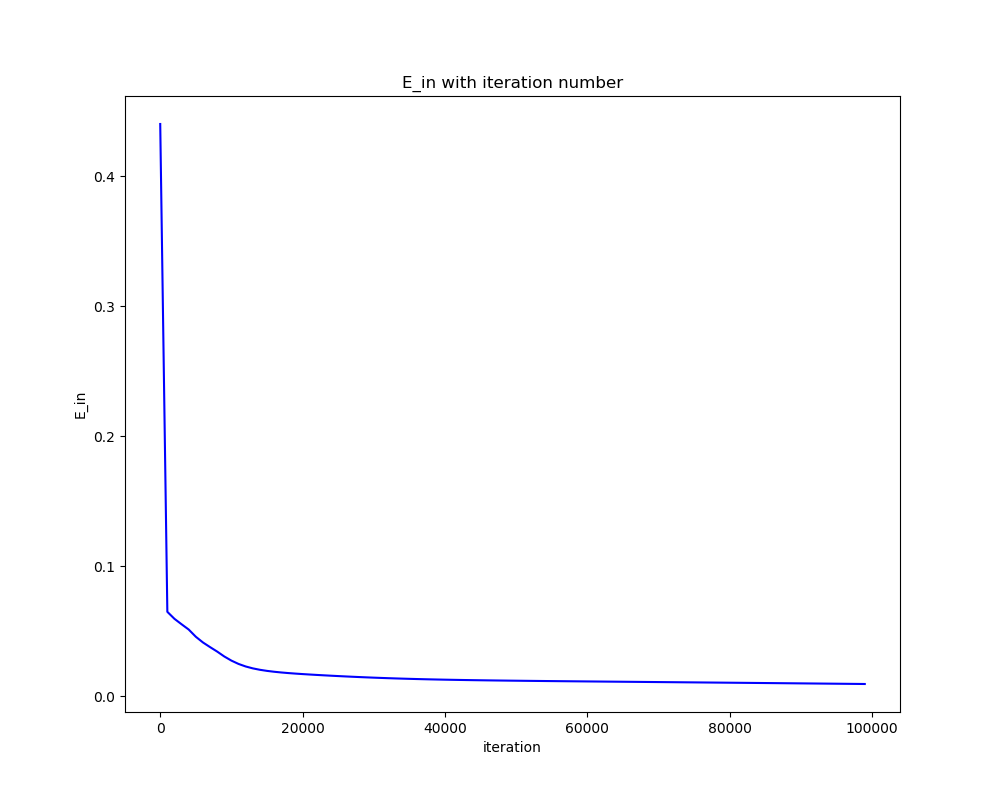
\includegraphics[height=9cm]{p2a1.png}}
	\end{figure}
	\newpage
	\begin{figure}[htb] 
			{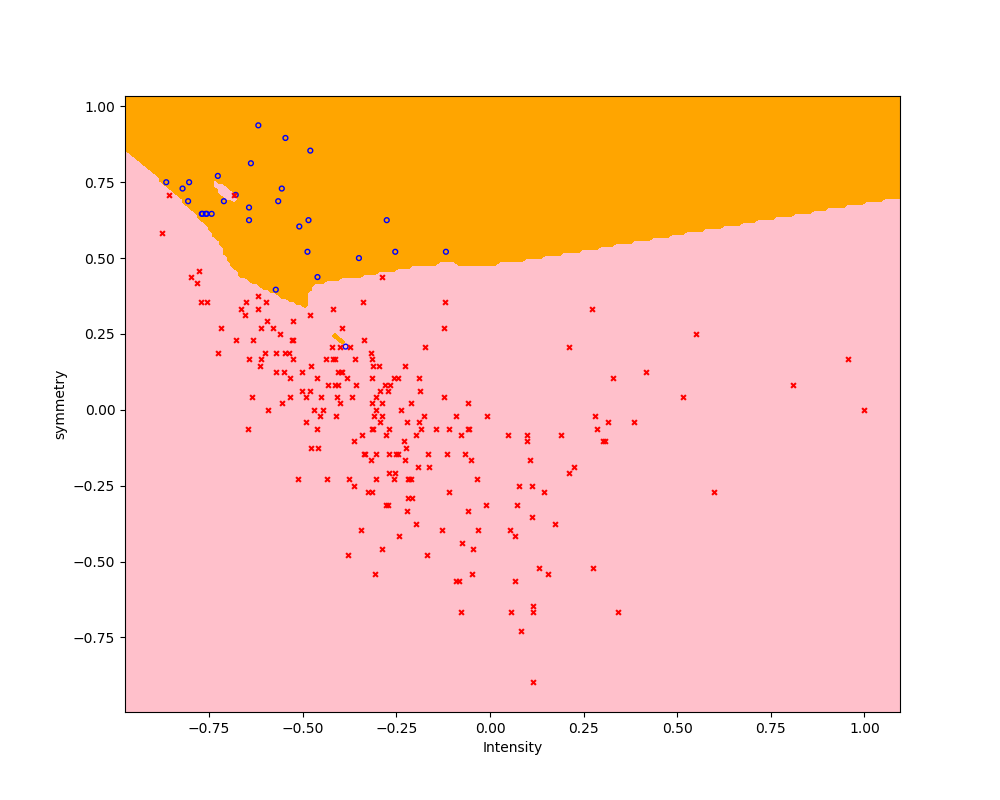
\includegraphics[height=9cm]{p2a2.png}}
	\end{figure}
	\item \ \begin{figure}[htb] 
			{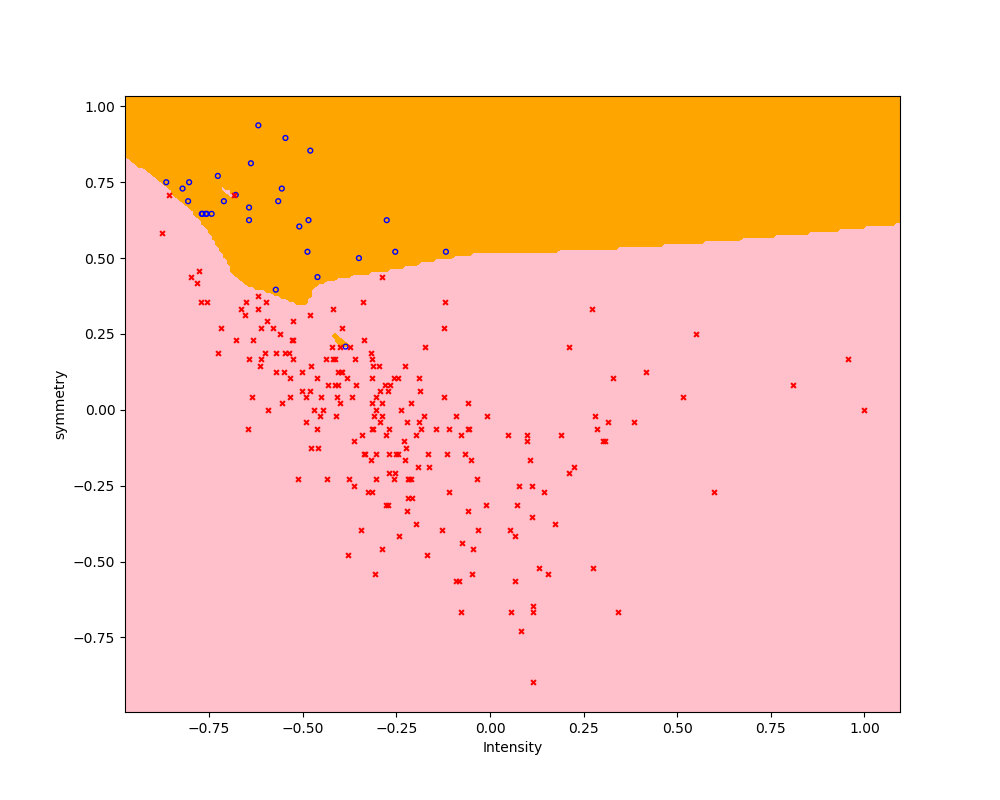
\includegraphics[height=8cm]{p2b.png}}
	\end{figure}
	\newpage
	\item \ \begin{figure}[htb] 
			{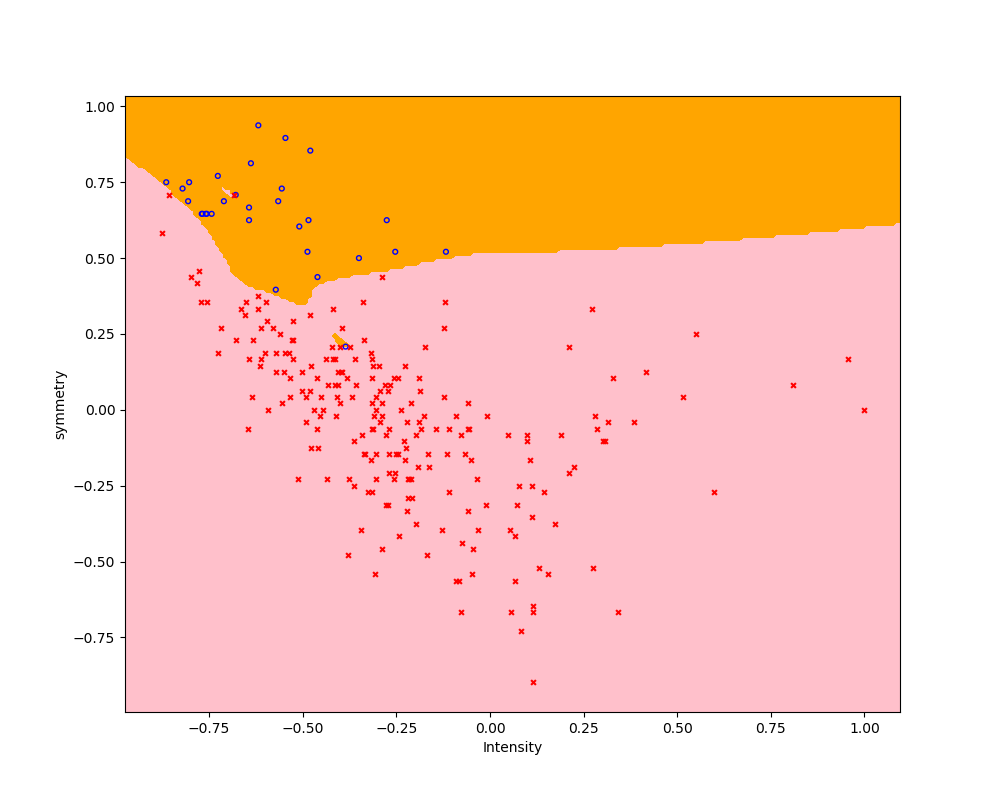
\includegraphics[height=9cm]{p2c.png}}
	\end{figure}
\end{enumerate}
\newpage
\noindent{\bf Problem 3}
\begin{enumerate} [(a)]
	\item \ \begin{figure}[htb] 
			{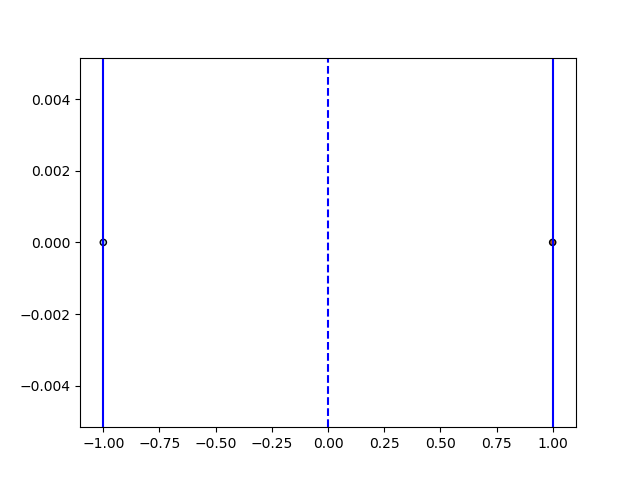
\includegraphics[height=8cm]{p3a.png}}
	\end{figure}
	x = 0
	\item\ \begin{figure}[htb] 
      {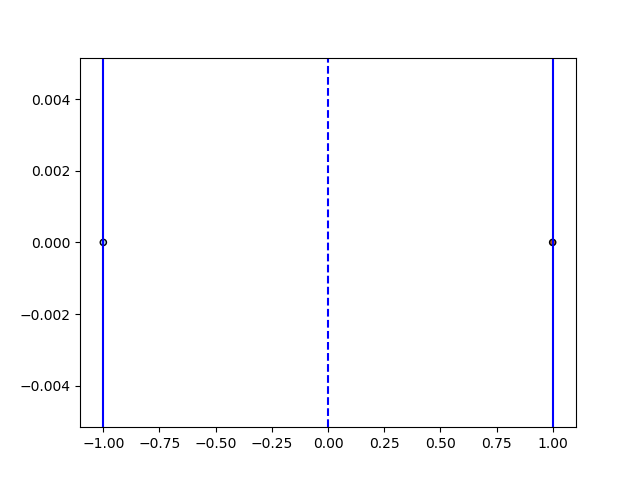
\includegraphics[height=8cm]{p3a.png}}
  \end{figure}
  \newpage
	\item\ \begin{figure}[htb] 
			{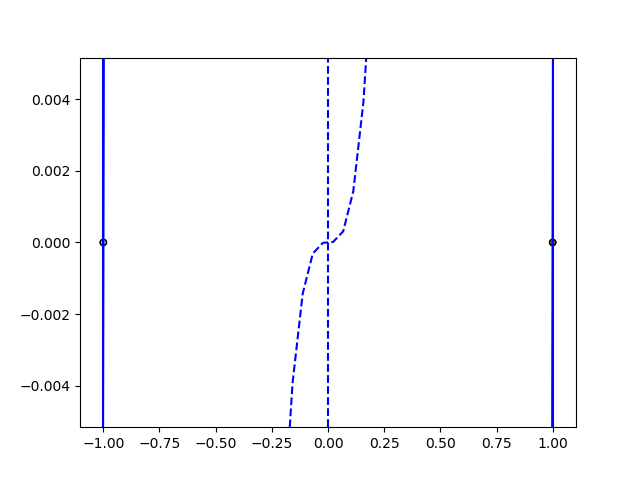
\includegraphics[height=8cm]{p3c.png}}
	\end{figure}
  z1 = [1, 0], y1 = 1, z2 = [-1, 0], y2 = -1
	\item $F=x_0^{3}y_0^{3}-x_0^{3}y_1-x_1y^3_{0}+x_1y_1+x_0x_1y_0y_1$

	\item $h(x)=sign(x^3-y)$
\end{enumerate}
\newpage
\noindent{\bf Problem 4}
\begin{enumerate} [(a)]
	\item small C = 0.001:\begin{figure}[htb] 
			{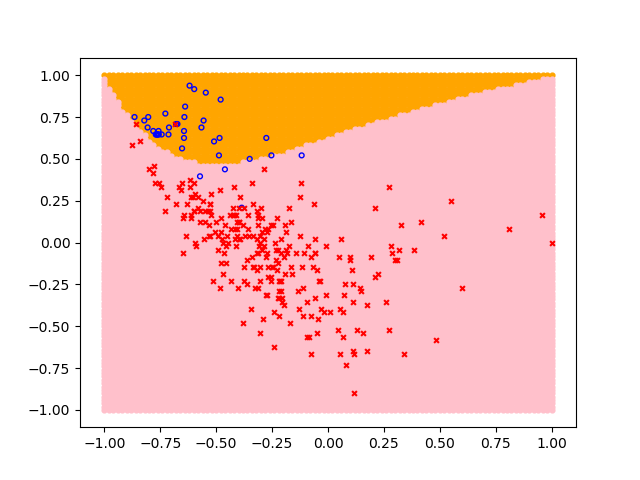
\includegraphics[height=8cm]{p4a1.png}}
	\end{figure}\\
	large C = 100:\begin{figure}[htb] 
			{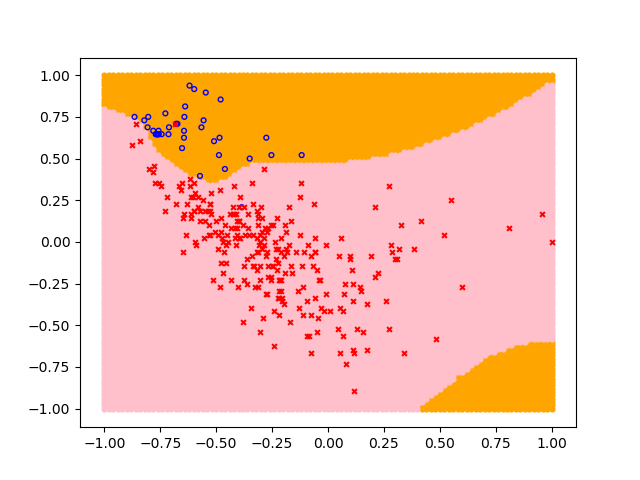
\includegraphics[height=8cm]{p4a2.png}}
	\end{figure}\\
	\newpage
	\item Generally, a large C can produce a result with high complexity. However, when C is too large, underfitting happened.
	\item C = 100 has the lowest $E_{test} = 0.01278$ \begin{figure}[htb] 
			{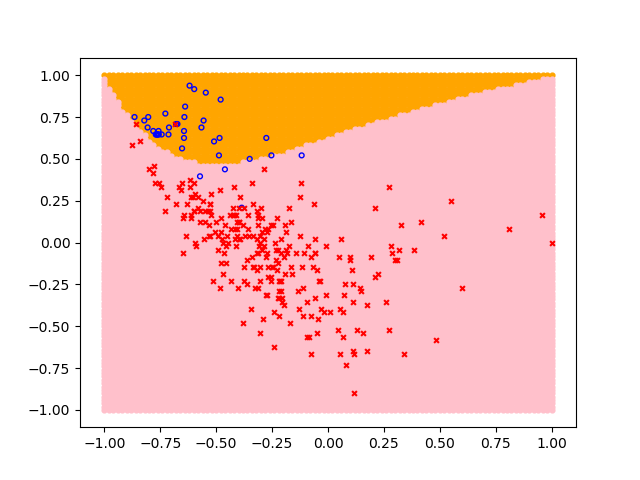
\includegraphics[height=8cm]{p4a1.png}}
	\end{figure}
\end{enumerate}
\noindent{\bf Problem 5}
$E_{test}$ for five methods:

\begin{tabular}{ll}
             & $E_{test}$ \\
Linear Model & 0.030669  \\
KNN          & 0.0202267  \\
RBF          & 0.0092242  \\
Neural network & 0.02867\\
SVM          & 0.01278
\end{tabular}\\
Above five $E_test$ are quite small, and RBF model produced the best boundary with the smallest $E_test$. The reason could be that in my case, RBF model use relatively large K value of 44, hence the decision boundary is much more strict than other methods.
\end{document}
\end{document}